\subsection{Südkamerun}\label{sec:Kamerun}

Das nordwestlich an das Arbeitsgebiet angrenzende südliche Kamerun zählt zu den gegenwärtig mit am besten erforschten Regionen innerhalb Zentralafrikas, neben dem Norden Gabuns (Kap.~\ref{sec:Gabun}) sowie dem Niederkongo (Kap.~\ref{sec:Niederkongo}).\footnote{Zur Geschichte der archäologischen Erforschung Südkameruns siehe auch \textcite[7--9]{Seidensticker.2010b}.} Zwischen 1925 und 1978 wurden durch \textcites{Jauze.1944}{Jauze.1944b}{Jauze.1948} im Umland der Hauptstadt Yaoundé erste Grabungen durchgeführt, die unter anderem 1940 zur Entdeckung der Fundstelle Obobogo führten \parencite[nach][458]{Clist.1990}. Ab den 1980er Jahren schlossen sich systematische Feldarbeiten unter der Leitung von Pierre \textcites{Maret.1980}{Maret.1982} an, in deren Rahmen die Fundstelle Obobogo erneut lokalisiert und neuere Grabungen durchgeführt werden konnten \parencite{Claes.1985}. In den \textit{Grassfields} Westkameruns wurden eine Reihe Abris archäologisch erforscht. Eine der umfangreichsten Sequenzen vom späten Pleistozän bis ins Holozän konnte an der Fundstelle Shum Laka erfasst werden.\footnote{Siehe \textcites{Asombang.1988}{Asombang.1992}{Cornelissen.1996}{Cornelissen.2003}{deMaret.1995}{Maret.1996}{Lavachery.1996}{Moeyersons.1996}.} Die ursprünglich mikrolithische \textit{Later Stone Age} (LSA) Steingeräteindustrie des Platzes wandelt sich im 5. Jt.~v.~Chr. zu einer makrolithischen Industrie, die auch geschliffene Steinwerkzeuge sowie Keramik umfasst und in Anlehnung an \textcite{McIntosh.1988} als \textit{Stone to Metal Age} \parencite[SMA;][213]{Lavachery.2001} beziehungsweise \textit{Stone to Metal Period} \parencite[SMP;][279]{Maret.1996} systematisiert wird. Diese überdauert bis zum Beginn der Eisenzeit im 4.~Jh.~v.~Chr. (ebd. 278). Die Keramik dieser obersten, stark durchmischten Schicht zeichnet sich durch \textit{knotted strip} (21.1) sowie \textit{twisted string} Roulette (21.2) aus. Die Region um die Hauptstadt Yaoundé war weiterhin ein Schwerpunkt der archäologischen Forschung in Kamerun und in den späten 1980er und frühen 1990er Jahren wurden eine Reihe weiterer Fundstellen entdeckt und untersucht \parencite{Essomba.1989}. Im Zuge der neuen Feldarbeiten entstanden eine Reihe von Promotionsschriften, so jene von Christine \textcite{Atangana.1988} zur Fundstelle Okolo, die Arbeit von Christoph \textcite{MbidaMindzie.19951996} über die Fundstellen Nkang und Ndindan sowie die Bearbeitung mehrere Fundstellen südlich des Sanagas durch Martin \textcite{Elouga.20002001}.

Die Arbeiten im Zentrum des Landes rückten vornehmlich die keramischen Formen des Fundplatzes Obobogo in den Mittelpunkt der Betrachtungen, da sie den Beginn der regionalen Sequenz bilden. Die Keramik aus Obobogo zeichnet sich durch flachbodige hohe Gefäße mit leicht geschweiften Wandungen sowie Wiegebanddekor und gerillten Rändern aus \parencite{Claes.1985}. Das Dekor ist häufig flächig über alle Gefäßteile hinweg angebracht. Neben der Keramik fanden sich auch Steinartefakte sowie Schlacke, was zumindest \enquote{eine Phase gleichzeitiger Verwendung lithischer und metallener Gerätschaften} andeutet \parencite[258f.]{Wotzka.1995}. Viele der vorliegenden Radiokohenstoffdatierungen aus Obobogo wurden im Labor in Hannover untersucht und weisen ähnliche starke Schwankungen auf, wie die Datierungen aus dem Inneren Kongobecken (siehe Kap.~\ref{sec:ICB_StilGrDatierungen}, Tab.~\ref{tab:14C_InnerCongo_Lab_Representation}). Auch wurden seinerzeit \enquote*{bulk samples} gebildet indem Probenmaterial vermischt wurde, um ausreichende Mengen Kohlenstoff für die Datierung zu erhalten \parencite[723]{Clist.20042005}. Die vorliegenden Daten streuen zwischen dem 24.--16.~Jh.~v.~Chr. (Hv-11046) sowie dem 2.~Jh.~v.~Chr.--2.~Jh.~n.~Chr. \parencites[Hv-10832;][147]{deMaret.1985b}[219f.]{Clist.1986}[nach][249 Anm. 21]{Wotzka.1995}. Von den insgesamt 13 Datierungen wurden nur lediglich drei nicht in Hannover untersucht (Lv-1394, Lv-1395, Lv-1432). Diese drei Datierungen decken eine Zeitspanne vom 8.~Jh.~v.~Chr. bis zum 3.~Jh.~n.~Chr. ab. Durch \textcite{Claes.1985} erfolgte lediglich eine grobe Aufarbeitung der Funde, so dass gesicherte Aussage nur bedingt möglich sind. Neben der Fundstelle in Obobogo selbst, fanden sich Vertreter dieses Stils auch in Avoh \parencite{Elouga.20002001}, Ndindan und Nkang \parencite{MbidaMindzie.19951996} sowie Okolo \parencites{Atangana.1988}[siehe][249 Abb.~133]{NlendNlend.20132014}. 

Der direkt an das Arbeitsgebiet anschließende Südosten Kameruns hat im Vergleich zum Zentrum des Landes sowie dem Südwesten vergleichsweise wenig Forschungsaktivität gesehen. Im Jahr 1997 nahm \textcite{Eggert.2002} die in dieser Arbeit präsentierten Feldarbeiten im Norden der Republik Kongo, entlang der Flüsse Sangha und Ngoko durch Prospektionen im Südosten Kameruns wieder auf. Aufgrund aufschlussreicher Funde entlang des Sanaga verschoben sich die Prioritäten dieser Feldarbeiten sukzessive in den Südwesten Kameruns. So wurden 1998/99 umfangreiche Grabungen im nahe der Mündung des Sanaga gelegenen Mounako durchgeführt. Das ebenfalls unter der Leitung von Manfred Eggert durchgeführte Teilprojekt \enquote*{Wandel der Umwelt und Kultur: Savanne, Regenwald und Kultur im südlichen und östlichen Kamerun} der 2004 begründeten DFG-Forschergruppe 510 \enquote{Ökologischer Wandel und kulturelle Umbrüche in West- und Zentralafrika} führte umfangreiche Feldarbeiten in Südkamerun durch. Obschon der Osten des Landes einige Untersuchungen erfahren hatte, lag auch der Fokus dieses Projektes auf dem Südwesten Kameruns. Gegenwärtig informiert lediglich ein Vorbericht über die Ergebnisse der Prospektionen des Tübinger Projektes im Südosten Kameruns (ebd. 510f.). Die Region um Moloundou am Ngoko erwies sich als äußerst spärlich besiedelt. Die für die Region zur Verfügung stehenden, auf Basis von Luftaufnahmen entstanden Karten deuten durch häufige Vermerke von Ölpalmen, die als indirekter Anzeigen für potentielle menschliche Aktivität angesehen werden können, an, dass dies in historischer Zeit deutlich anders war und die Region dicht besiedelt gewesen sein kann. Auch aufgrund hoher Wasserstände erbrachte die Prospektion des Jahres 1997 im Südosten Kameruns keine Hinweise auf frühe Keramik. Die archäologischen Funde neuerer Forschungsaktivitäten in der Region \parencite{MorinRivat.2014} sind gegenwärtig noch nicht abschließend bearbeitet.

\begin{figure*}[p]
	\centering
	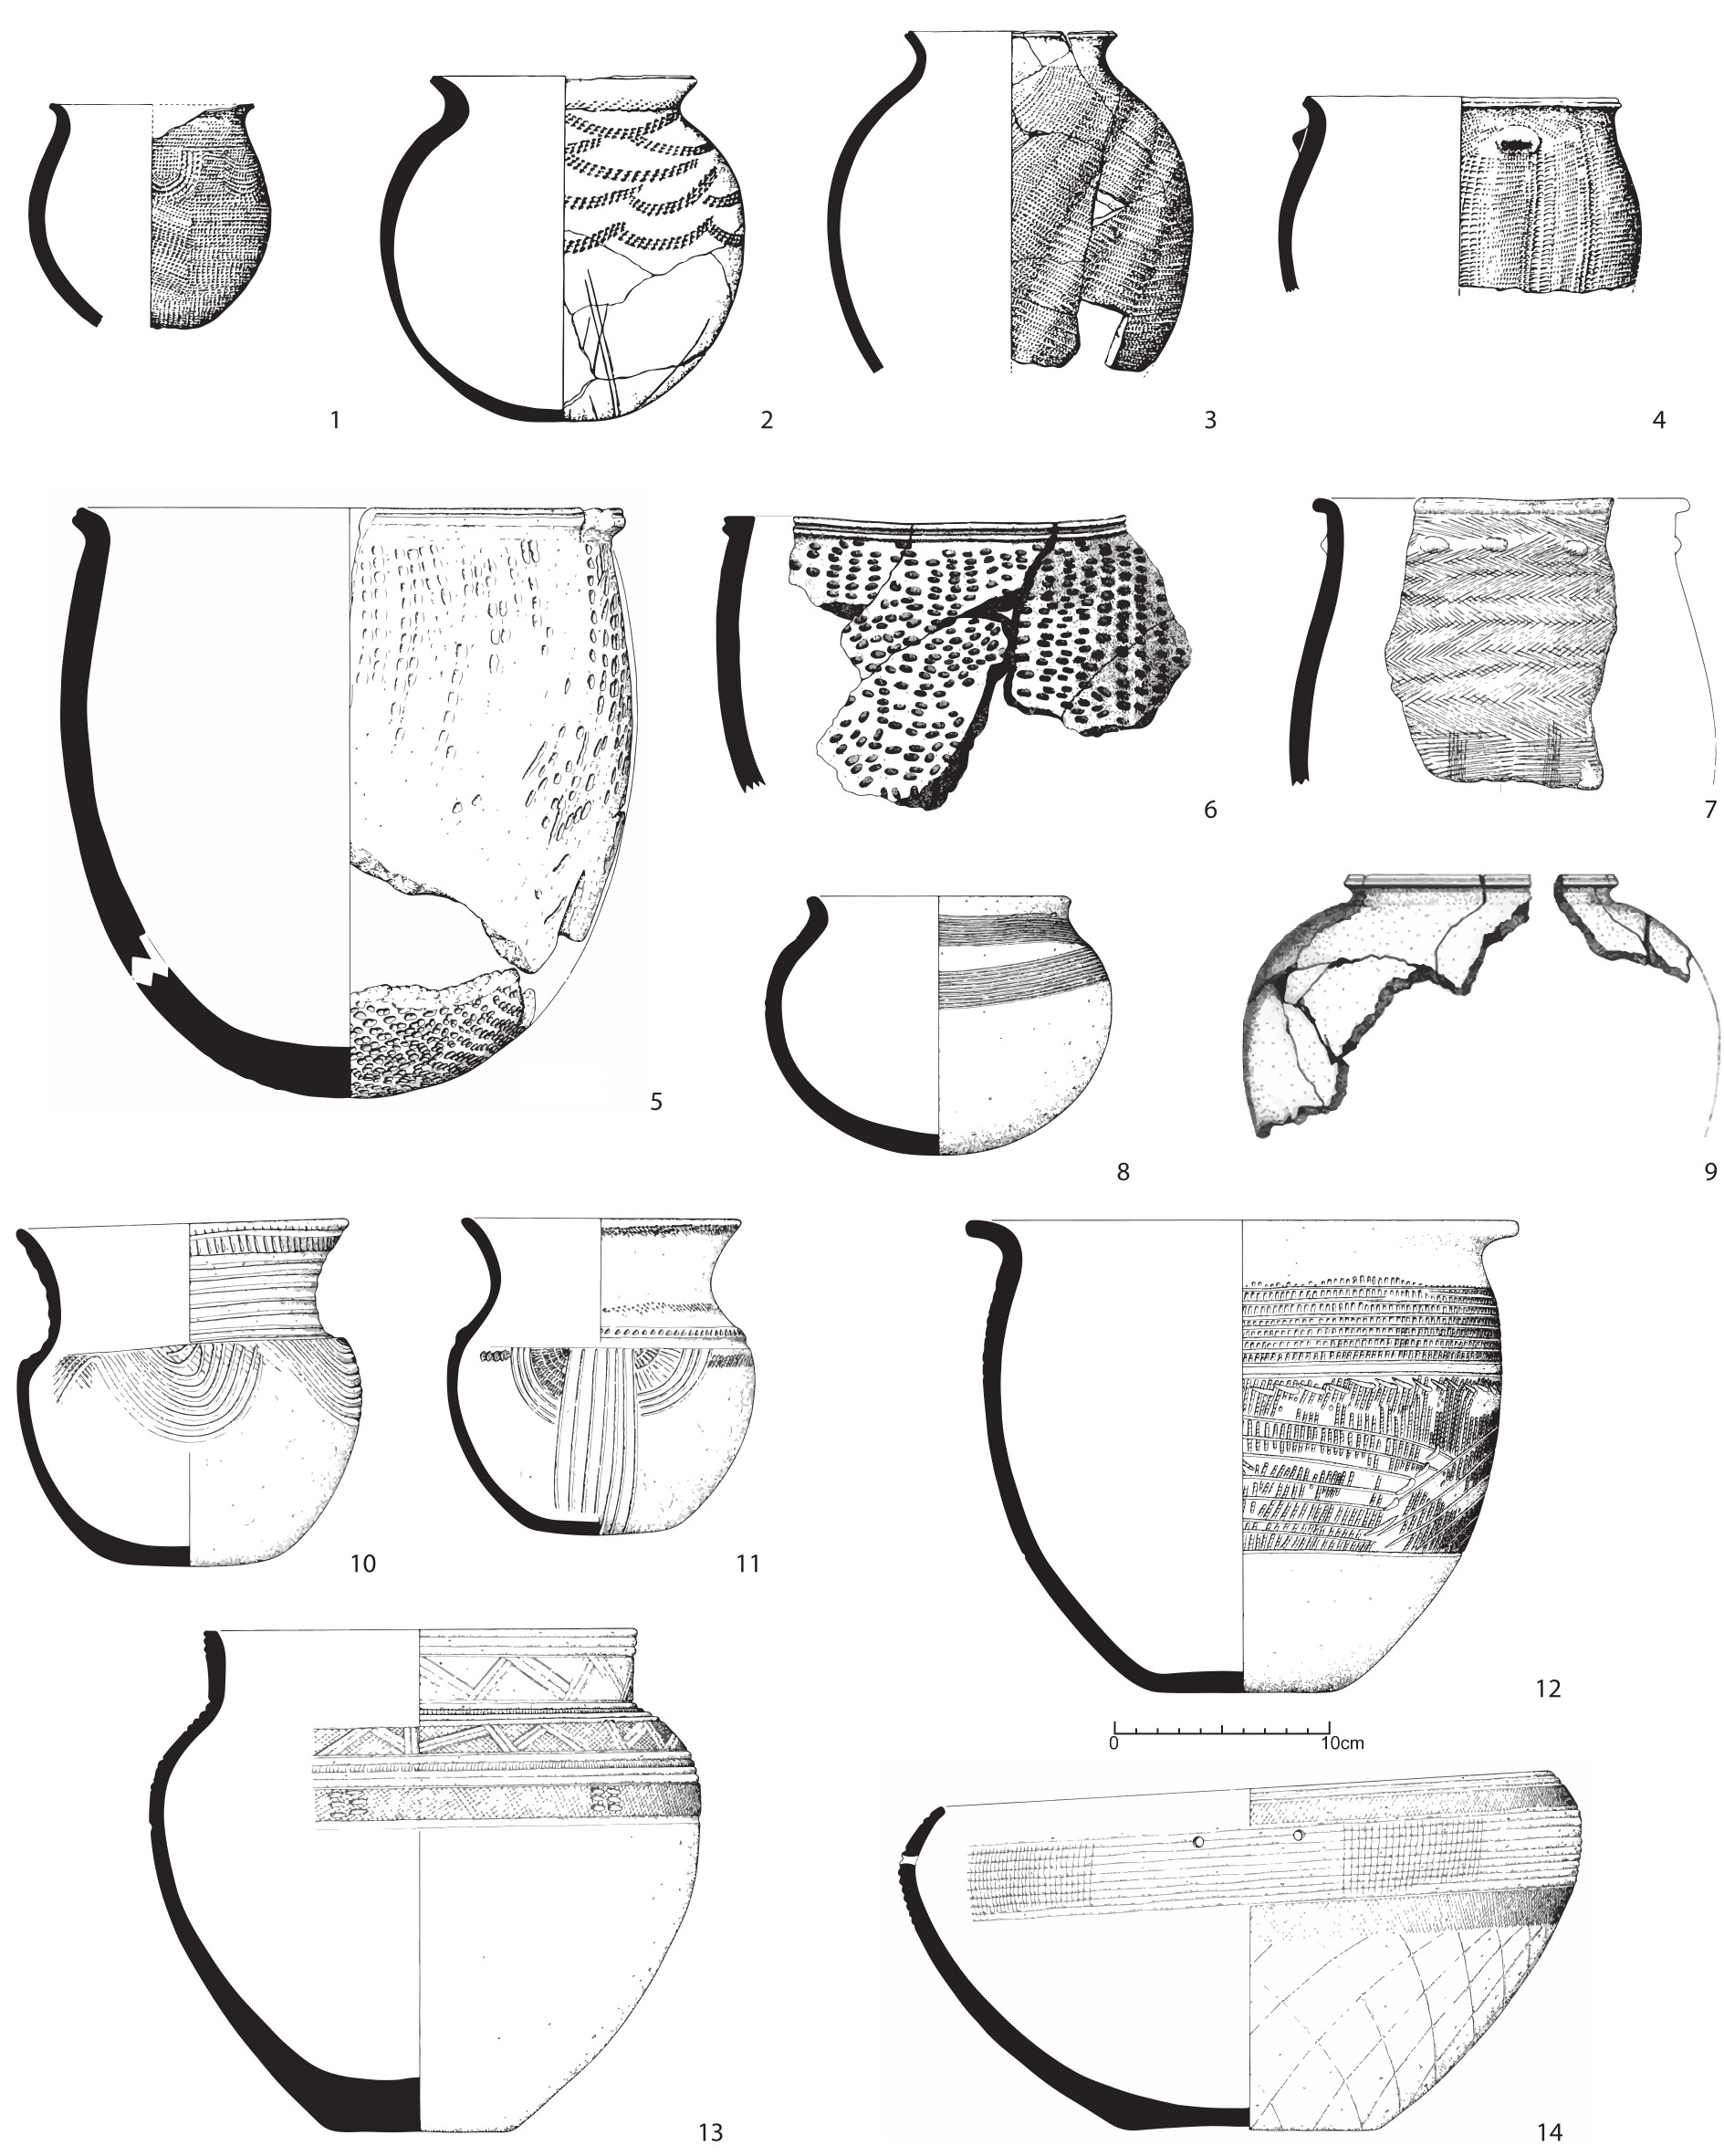
\includegraphics[width = \textwidth]{lit/Kamerun_Typen.pdf}
	\caption{Südwestkamerun: Regionale Sequenz der frühen Eisenzeit nach \textcites{GouemGouem.20102011}{NlendNlend.20132014}.\\{\footnotesize 1--4: Obobogo-Gruppe \parencites[Taf. 25.1--2, 37.1, 39.2]{Claes.1985}[632 Abb.~43.4]{deMaret.2013}; 5--7: Bissiang/Malongo-Gruppe \parencites[34 Abb.~14]{Oslisly.2001c}[282 Abb.~3.2, 287 Abb.~7.3]{Eggert.2006b}; 8--9: Mpoengu/Bwambé-Gruppe \parencites[282 Abb.~3.7]{Eggert.2006b}[252 Abb.~114.2]{NlendNlend.20132014}, 10--13: Akonètye-Gruppe \parencite[195 Abb.~10.2--5]{Meister.2008b}; 14--15: Campo-Gruppe \parencite[98 Abb.~5.6, 182 Taf.~12.2, 184 Taf.~14.4]{Eggert.2016}.}}
	\label{fig:swCameroon_Sequence}
\end{figure*}

Die in den letzten Jahrzehnten wohl am besten untersuchte Region Kameruns ist das Umland von Kribi sowie der Küstenabschnitt zwischen Kribi und Campo. Vor allem die Surveys im Zuge der Errichtung der die Erölfelder in Kome (Tschad) mit Kribi verbindenden Erdölpipeline\footnote{Die Arbeiten des \enquote*{Pipeline}-Projektes erbrachten zahlreiche neue Fundstellen entlang eines knapp 1100\,km langes Transektes. Im Zuge dieser Zusammenstellung flossen lediglich die Funde aus dem südwestlichen Kamerun ein \parencites[siehe][]{Lavachery.2005}{Lavachery.2010}.} sowie Prospektionen und Grabungen unter der Leitung von Richard Oslisly\footnote{Siehe \textcites{Oslisly.2006}{Oslisly.2006d}.} und solche des Tübinger Kamerun-Projektes \parencites{Eggert.2006b}{Meister.2008b} verdichteten die archäologische Karte des südwestlichen Kameruns merklich. Im Zuge der Promotionsarbeiten von Bienvenu \textcite{GouemGouem.20102011} und Pascal \textcite{NlendNlend.20132014} kam es zu einer abweichenden nomenklatorischen Beschreibung der jeweils gleichen archäologischen Phänomene. Die ältesten keramischen Zeugnisse werden von \textcite[330ff.]{GouemGouem.20102011} der Bissiang-Gruppe zurechnete, während die gleichen Formen von \textcite[233--249]{NlendNlend.20132014} einer Malongo genannten Gruppe zugewiesen werden. Die entsprechende Keramik zeichnet sich hohe, ovaloide Gefäße mit flächiger Fisch-Grät-Verzierung, Kammwiegeband sowie häufig kurz ausbiegenden, gerillten Rändern aus \parencites[337 Abb.~11.6]{GouemGouem.20102011}[237--239 Abb.~102--104]{NlendNlend.20132014}. Vertreter dieser Keramik fanden sich in Bissiang, Dombè, Malongo, Bwambé-Sommet, Abang Minko'o und Mpolongwé-Kribi sowie Campo \parencites[336, 339 Karte 1.6]{GouemGouem.20102011}[254]{NlendNlend.20132014}{Seidensticker.2010b}. \textcite[336 Abb. 10.6]{GouemGouem.20102011} gibt für die Bissiang-Gruppe auf Basis von je zwei Datierungen aus Bissiang (Beta-182548, Beta-182549) und Dombe (Beta-182546, Beta-182547) ein Alter zwischen dem 11.--4. Jh.~v.~Chr. an, wobei ohne die älteste Probe Beta-182549 lediglich eine Spanne zwischen dem 8.--4. Jh.~v.~Chr. angegeben werden kann (ebd. 336 Abb. 10.6). Für die der Bissiang-Keramik entsprechende Malongo-Gruppe werden von \textcite[255 Abb.~116]{NlendNlend.20132014} 12 Datierungen genannt, die einen Zeitraum vom 11.~Jh.~v.~Chr. bis in das 1.~Jh.~v.~Chr. abdecken. Die Malongo-Gruppe wird von \textsc{Nlend Nlend} (ebd. 247) als Teil der vielgestaltig systematisierten, ähnlich frühen Keramik in Kamerun und Gabun angesehen. \textcite[632 Abb.~43.3]{deMaret.2013} kartiert diese unterschiedlich bezeichneten Gruppen, die jedoch alle mehr oder weniger das gleiche keramische Phänomen abbilden gemeinsam, unter der Bezeichnung \enquote*{Diverse verwandte Traditionen}.

Des Weiteren beschreibt \textcite[255]{NlendNlend.20132014} einen ab dem frühen 7.~Jh.~v.~Chr. aufkommenden Stil, den er als Bwambé-Gruppe bezeichnet. Das Formenspektrum entspricht dabei den von \textcite[352--358, 354 Abb.~17.6]{GouemGouem.20102011} als Mpoengu-Gruppe subsumierten Inventaren. Beide zeichnen sich durch rundbauchige Gefäße mit in horizontalen Bändern organisiertem Dekor und kurzen, ausbiegenden Rändern aus \parencite[ebd. 352--358, 354 Abb.~17.6; ][252 Abb.~114]{NlendNlend.20132014}. Während \textcite{GouemGouem.20102011} diese Funde an den Beginn der regionalen Eisenzeit stellt\footnote{\textcite[349f.]{GouemGouem.20102011} setzt den Beginn der Eisenzeit im südwestlichen Kamerun um 400~v.~Chr. an und führt als Beleg Funde eines Ofen aus Makouré~I sowie Fragmente von Tuyères aus Kpwé-Monekpwé an. Ebenfalls in die Frühe Eisenzeit, die mit einem Bruch in der Sequenz einhergehen, werden von \textsc{Gouem Gouem} (ebd. 350) Funde aus Talla (TAL~II-BK), Mpoengu (MPO-I-A) sowie Bwambé (Bwambé-Est) eingeordnet.}, die bei ihm erst im 4. Jh.~v.~Chr. beginnt (ebd. 349f.), repräsentiert die Bwambé-Gruppe bei \textcite{NlendNlend.20132014} noch einen Zustand, der er einer \textit{Stone to Metal Age} (SMA) zuordnet. Die Bwambé-Keramik wird von \textsc{Nlend Nlend} (ebd. 256 Abb.~117) bis in das frühe 2. Jh.~n.~Chr. datiert, während die von ihm beschriebene, ältere Malongo-Gruppe bis in das späte 1. Jh.~v.~Chr. bestanden haben soll (ebd. 255 Abb.~116). Auffällig in der Analyse von \textcite{NlendNlend.20132014} ist der hohe Anteil durchmischter Inventare.\footnote{Sieben Gruben weisen ausschließlich Keramik auf, die von \textcite{NlendNlend.20132014} der Malongo-Gruppe zugerechnet wird (Bissiang A und B; Dombé A und B, Malongo 2 sowie Mpolongwé-Kribi 15 und 22), während sieben Gruben ausschließlich Material der Bwambé-Gruppe enthalten (Bwambé 1, 2, 4, 9 und 11 sowie Mpoengu I-A und Talla II BK). Elf weitere Gruben enthalten Formen beider Gruppen (Bwambé 12, 16, 17, 19, 32, 33 und 34 sowie Mpolongwé-Kribi 8, 23, 31 und 36; ebd. 257 Tab.~44). \textsc{Nlend Nlend} (ebd. 257 Tab.~44) wertet die Inventare aus den Gruben 1 und 2 in Bwambé, die beide jeweils 97,99 beziehungsweise 86,19\,\% Keramik der Bwambé-Gruppe enthalten, als durchmischt, während Inventare mit deutlich geringeren Anteilen der Malongo-Keramik vollständig dieser zugerechnet werden. Hierzu zählen die Inventare aus den Gruben 16 (47,05\,\% Malongo-Keramik), 17 (68,6\,\% Malongo-Keramik) sowie Grube 19 aus Bwambé, die nur 27,53\,\% Malongo-Keramik enthielt. Die notwendigen Korrekturen sind in die weiter oben genannten Zahlen bereits eingeflossen.} Bereits im Inventar aus Grube 31 in Mpolongwe-Kribi, welches in das 9.--7.~Jh.~v.~Chr. datiert und zu den ältesten datierten Grubeninventaren der von \textcite{GouemGouem.20102011} und \textcite{NlendNlend.20132014} untersuchten Region gehört, findet sich Keramik, die von \textsc{Nlend Nlend} (ebd. 257 Tab.~44) der Bwambé-Gruppe zugerechnet wurde. Auch die ins 9.--5.~Jh.~v.~Chr. datierte Grube 17 aus Bwambé enthält knapp 1/3 nicht der Malongo-Gruppe zurechenbare Funde. 

Eine zweite, entwickeltere Phase der frühen Eisenzeit sieht \textcite[363--369, 368 Abb.~30.6]{GouemGouem.20102011} durch die Keramik der Bidjouka-Gruppe repräsentiert, die ein tief in die Oberfläche eingearbeitet, im Profil U-förmige Riefen sowie sowie Kammwiegeband aufweist. Dieser Stil datiert zwischen das 1.--7.~Jh.~n.~Chr. (ebd. 371 Abb.~33.6) und ist zeitgleich mit der Belegung des Gräberfeldes in Campo und der dort angetroffenen Keramik, die eine eigene Stilgruppe repräsentiert \parencite[98 Abb.~5.6]{Eggert.2016}.

Die in das 1. Jh.~v.~Chr. bis 3. Jh.~n.~Chr. datierenden, 1998/99 an der Mündung des Sanaga ausgegrabenen Befunde aus Mouanko-Lobethal, dem benachbarten Mouanko-Epolo sowie dem auf der gegenüberliegenden Flussseite gelegenen Yatou\footnote{In Mouanko-Lobethal wurde unter anderem ein aus neun sich überlagernden Gruben bestehender Komplex sowie vier weitere Gruben untersucht \parencite[513]{Eggert.2002}.} erbrachten keramische Inventare, die deutliche Bezüge zur Keramik der Gräber in Campo \parencite[98 Abb.~5.6]{Eggert.2016} sowie einer zeitgleichen Grube aufwiesen \parencite[161 Abb.~3.5--10]{Seidensticker.2010c}. Die Inventare zeichnen sich durch offene Schalenformen sowie Gefäße mit geschweifter Wandung, kurzem Hals und ausbiegenden Rändern aus \parencite[514--519 Abb.~7--12]{Eggert.2002}. Das Dekor setzt sich vornehmlich aus Rillen oder Riefen sowie Kammeindrücken zusammen. Gefäße aus Grube 1 der am südlichen Ufer des Sanaga gelegenen Fundstelle Yatou weisen hingegen schwache Ähnlichkeiten zur den diagnostischen Schalen der Pikunda-Munda-Gruppe auf (Kap.~\ref{sec:PKM-Gr}). Wie diese, haben die Gefäße aus Yatou einen scharfen Knick zwischen Ober- und Unterteil und einen runden Boden. Die Verzierung besteht wie bei der Pikunda-Munda-Gruppe aus horizontalen Bändern wobei die Gefäße aus Yatou vornehmlich Kammeindrücke, in einem Fall ein aus einzelnen horizontalen Kammeindruck-Bändern gebildetes Fischgrätmuster, aufweisen und die Gefäßunterteile unverziert bleiben. Auch die Randgestaltung lässt Parallelen zwischen der Keramik aus Yatou und jener der Pikunda-Munda-Gruppe erkennen: die grundsätzlich ausbiegenden Ränder weisen, die auch bei der Pikunda-Munda-Keramik beobachtbaren, einbiegenden Randlippen auf (vergleiche Taf.~41.18, 45.2, 50.7, 52.6 mit ebd. 519 Abb.~12.2--3).\clearpage

Der jüngere Abschnitt der frühen Eisenzeit im südwestlichen Kamerun, im Anschluss an die Mpoengu-Gruppe, wird von \textcite[379f.]{GouemGouem.20102011} in zwei große Phasen unterteilt: eine erste Phase vom 1.--4.~Jh.~n.~Chr. mit Funden aus Akonétyé, Minyin, Mouanko-Lobethal sowie Campo und eine zweite Phase zwischen dem 4.--10.~Jh.~n.~Chr. mit Funden aus Bidjouka, Kribi-Mission catholique, Talla, Mpoengu, Eboundja 3, Bidou I, Bwambé Beach und Boussibilinga. Eine in Mpoengu freigelegte Bestattung datiert in diese zweite Phase (ebd. 305--317, 384--389). Zur ersten Phase zählen auch die in das 1.--4.~Jh.~n.~Chr. datierenden Funde aus dem am Mboro-Fluss, nördlich von Ambam gelegenen Akonétye \parencite[184]{Meister.2008b}. Die untersuchten Bereiche der Fundstellen erbrachten nahezu zeitgleiche Gruben, jedoch zeigen sich zwischen den keramischen Inventaren einer nördlichen sowie einer unabhängigen südlichen Fundstellen deutliche formale Unterschiede. Die Gruben der südlichen Fundstelle waren zwischen 0,5--3,9\,m tief und enthielten Keramikobjekte, die sich durch hohe, leicht geschweifte Gefäße mit flachen Böden und ausbiegenden Rändern auszeichnen (ebd. 188 Abb.~5). Die Stücke sind vor allem mittels horizontal um die Gefäße laufenden, breiten in Wiegebandtechnik erzeugten Bändern sowie Rillen und kleineren Eindruck-Reihen verziert. Die zeitgleiche nördliche Fundstelle erbrachte eine komplett andersartige Keramik: gedrungenere Gefäße mit geschweifter Wandung und auffälligem Schulterabsatz. Ihr Dekor besteht aus horizontalen Rillen an vornehmlich langen, konvexen Halsbereichen sowie bogen- beziehungsweise girlandenförmigen Rillenbündeln unterhalb der Schulterabsätze (ebd. 195 Abb.~10). Die jeweiligen Grubeninventare der beiden Fundstellen von Akonétye sind formal in sich äußerst homogen, unterscheiden sich untereinander aber diametral. Der Keramik der nördlichen Fundstelle aus Akonétye entsprechendes Material fand sich auch im zirka 20\,km entfernt gelegenen Minyin (\textsc{Meister \& Eggert} 2008: 196 Abb.~11)\footnote{Die Funde aus Minyin datieren in das 1. Jh.~v.~Chr. bis 3. Jh.~n.~Chr. \parencite[189 Tab.~1]{Meister.2008b}.} sowie östlich von Sangmélima in Nkpwala-Esse \parencite{Meyer.2008}.